%%%%%%%%%%%%%%%%%%%%%%%%%%%%%%
% LATEX-TEMPLATE TECHNISCH RAPPORT
%-------------------------------------------------------------------------------
% Voor informatie over het technisch rapport, zie
% http://practicumav.nl/onderzoeken/rapport.html
% Voor readme en meest recente versie van het template, zie
% https://gitlab-fnwi.uva.nl/informatica/LaTeX-template.git
%%%%%%%%%%%%%%%%%%%%%%%%%%%%%%

%-------------------------------------------------------------------------------
%	PACKAGES EN DOCUMENT CONFIGURATIE
%-------------------------------------------------------------------------------

\documentclass{uva-inf-article}
\usepackage[english]{babel}
\usepackage[table,xcdraw]{xcolor}
\usepackage{float}
\usepackage{graphics}
\usepackage{pdfpages} 


% Relevant voor refereren vanaf blok 5
\usepackage{cite}
\usepackage[style=authoryear-comp]{biblatex}
\addbibresource{main.bib}

%-------------------------------------------------------------------------------
%	GEGEVENS VOOR IN DE TITEL
%-------------------------------------------------------------------------------

% Vul de naam van de opdracht in.
\assignment{Projectplan}
% Vul het soort opdracht in.
\assignmenttype{Projectplan}
% Vul de titel van de eindopdracht in.
\title{How people form beliefs about generics}

% Vul de volledige namen van alle auteurs in.
\authors{Bodi Boelé}

% Vul de corresponderende UvAnetID's in.
\uvanetids{11904089}

% Vul altijd de naam in van diegene die het nakijkt, tutor of docent.
\tutor{Dr. Patricia Mirabile}
% Vul eventueel ook de naam van de docent of vakcoordinator toe.
\docent{dhr. dr. R.G. (Rob) Belleman}
% Vul hier de naam van de PAV-groep  in.
\group{}
% Vul de naam van de cursus in.
\course{Afstudeerproject bachelor Informatica}
% Te vinden op onder andere Datanose.
\courseid{5062ABI18Y}

% Dit is de datum die op het document komt te staan. Standaard is dat vandaag.
\date{\today}

%-------------------------------------------------------------------------------
%	VOORPAGINA
%-------------------------------------------------------------------------------

\begin{document}
\maketitle

%-------------------------------------------------------------------------------
%	Inhoudsopgave
%-------------------------------------------------------------------------------
%-------------------------------------------------------------------------------
%	Achtergrond
%-------------------------------------------------------------------------------

\section{Background}
To be able to acquire the Bachelor of Computer Science, it is necessary to successfully complete the "Afstudeerproject Bachelor Informatica" - "Graduation project Bachelor of Computer Science". This project plan is part of the preparation of the graduation project. The graduation project discussed in this plan will contribute to a research project on the semantics of generic statements.

Generics are statements that express generalizations about the members of a kind, such as 'ducks lay eggs', 'tigers are striped', 'cars have radios' and 'ravens are black'. 'Bare' generic statements express useful generalizations, but it is difficult to come to an unambiguous conclusion on how these statements come about. There is no unique critical point where people tend to designate a statement as true. For example when people have to judge the statement "lions have manes", the predominant conclusion will be true, while less than 50\% of lions (only the older male lions) have manes. When asked about the statement "ticks spread Lyme disease" the predominant conclusion as well would be true, eventhough the statement is only true for 2.7\% \parencite{rivm_2019} of tick bytes that actually transfer the disease whereas 20\% of ticks carry the disease. These rather large differences in truth-conditions are described in \cite{leslie2011all}, where different types of predications are used to classify the generic statements.

\newpage
%-------------------------------------------------------------------------------
%	Projectdoelstelling
%-------------------------------------------------------------------------------
\section{Relevant readings}
The generic overgeneralization effect, as described by \cite{leslie2011all}, shows that  people tend to falsely (over)generalize statements. Another relevant research project is the project by \cite{tasimi2017differences} which concludes that "people’s
judgments about generic statements differ depending on whether the target category is
human or non-human. Generic judgments about human categories do not exhibit the same
negativity bias that generic judgments about non-human categories do." This research als suggests that it is "necessary to explore the cognitive processes underlying these
effects" which is part of the goal of the overarching research project of this project.

\cite{cimpian2010generic} also states that "generic statements require little evidence for acceptance" such as the previously mentioned tick example and other striking generics like "Rottweilers maul children" and "Lions eat people" eventhough these statements are only true for exceptional cases. In their conclusion they state that "Generic statements are often judged true based on weak evidence but
have implications that go far beyond what is needed to accept them." which underlines the importance of the parent research. 
The research done by \cite{khemlani2007ducks} is about how people interpret generic assertions, which is important to be able to understand how people form these assertions in the first place. 

%-------------------------------------------------------------------------------
%	Projectresultaat
%-------------------------------------------------------------------------------
\section{Research question}
The goal of this project is to implement software to be used for a scientific research project on how people form beliefs about generics. The result would then be an online experiment where participants are able to interact with the environment, discover information about the objects inside it and evaluate generic statements about those objects. 

The final result of this thesis will be an online hosted experiment that can be used for the aforementioned scientific research project. This will be published in a final thesis, along with the source code and the necessary documentation.

The research question of this project will be in line with the research project and therefor be: "How people form belies about generics."



%-------------------------------------------------------------------------------
%	Projectorganisatie
%-------------------------------------------------------------------------------
\section{Organisation}
\subsection{Method}
The project will be a combination of a literature review, to be able to understand the goal of the project. Together with setting up the experiments environment, executing the experiment in a limited form and submitting this instrument to be used in a bigger scale research project, by hosting it online.
\subsubsection{Communication}
\begin{itemize}
    \item Zoom - Planned meetings through Zoom, every Wednesday at 4pm.
    \item Email - For questions outside the Zoom meetings.
    \item Logbook - Keep track of progress made on a daily basis, available through GitHub
    \item Github - Keep track of coding and progress being made, as keeping files available at all times.
\end{itemize}

%-------------------------------------------------------------------------------
%	Projectplanning
%-------------------------------------------------------------------------------
\section{Planning}
The table below shows a graphical display of the proposed deadlines for the project.
\begin{table}[H]
\centering
\caption{Deadlines}
\label{my-label}
\begin{tabular}{cp{1cm}p{5cm}p{5cm}}
Date & Type & Assignment & Necessities  \\
\hline
April 2nd (23h59) & Personal & Project plan & Send to supervisor for approval \\
April 3rd (23h59) & Project & Project plan & Approval by project supervisor \\
April 24 (23h59) & Personal & First draft of the thesis & Send to supervisor for approval \\
May 1st (23h59) & Project & First draft of the thesis & Layout (Better if first chapter finished and sections of the other chapters have been set up)\\
May 29th (23h59) & Personal & "Go"/"no-go" version of the thesis & Send to supervisor for approval \\
June 5th (23h59) & Project & "Go"/"no-go" version of the thesis & Approval by project supervisor \\
June 15th (23h59) & Project & Final version of the thesis & Approval by project supervisor \\
June 15th (23h59) & Project & Delta document of the thesis & Briefly indicate the changes that have been made compared to the Go / No-go version of the thesis.
\end{tabular}
\end{table}

These deadlines can be used as a guide for the critical points of the project. Intermediate critical points have to be formed during the project itself. These intermediate points depend on the design and how this affects the overall flow of the project. Some critical points, such as that results must be in by the end of May. It is also important that the workload of the thesis itself is spread out throughout the project instead of postponing this till the very end. 
In conclusion, there is one extremely critical dependence which is the correct functioning of the code/software.

\subsection{GanttProject}
The GanttProject planning in figure \ref{fig:planning} has been included to be used as a guideline. (A full-page version has been added as Appendix 6.1)
\begin{figure}[H]
 \centering
 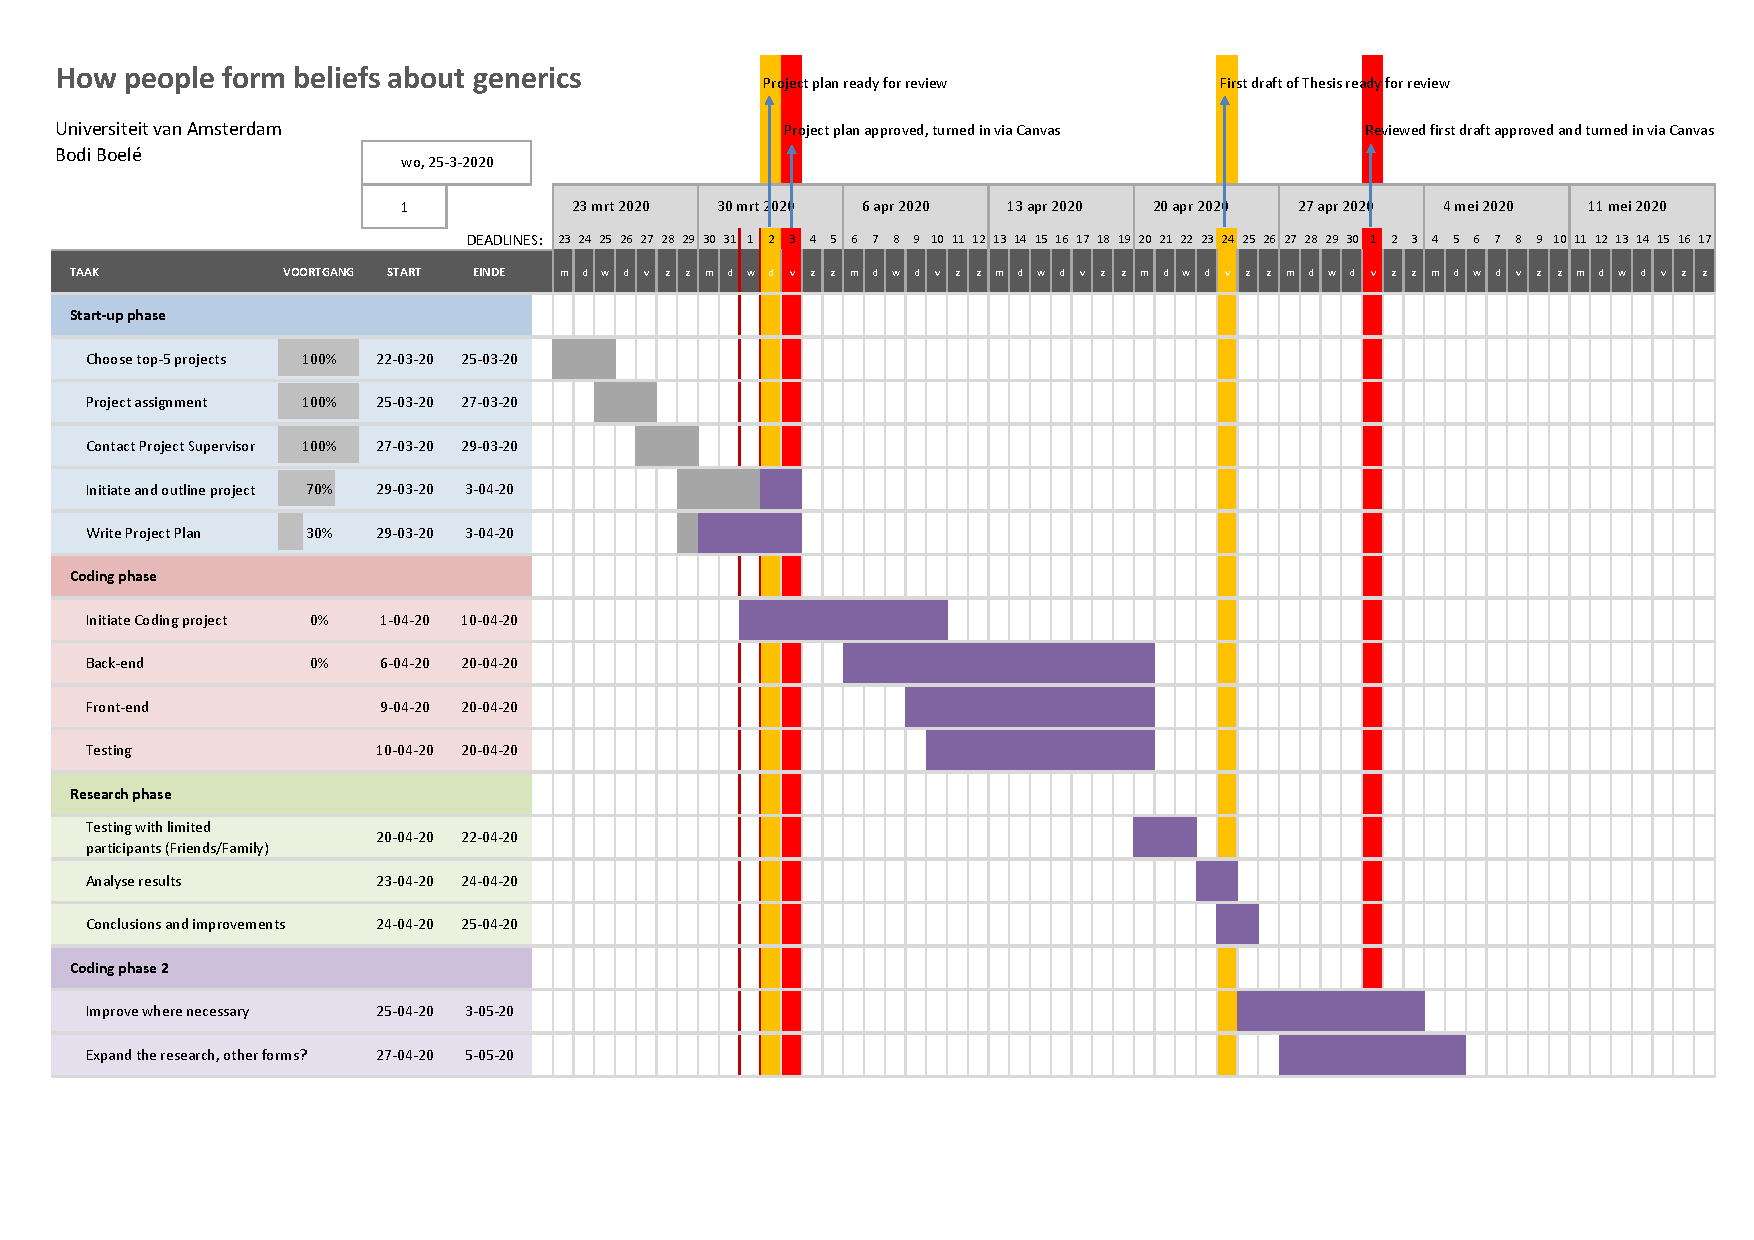
\includegraphics[page=1,width=1.1\textwidth]{Gant_planning_Afstudeerproject.pdf}
 \caption{GanttProject planning (d.d. 1-4)}
 \label{fig:planning}
\end{figure}

\printbibliography

\section{Appendix}
\subsection{GanttProject.pdf}
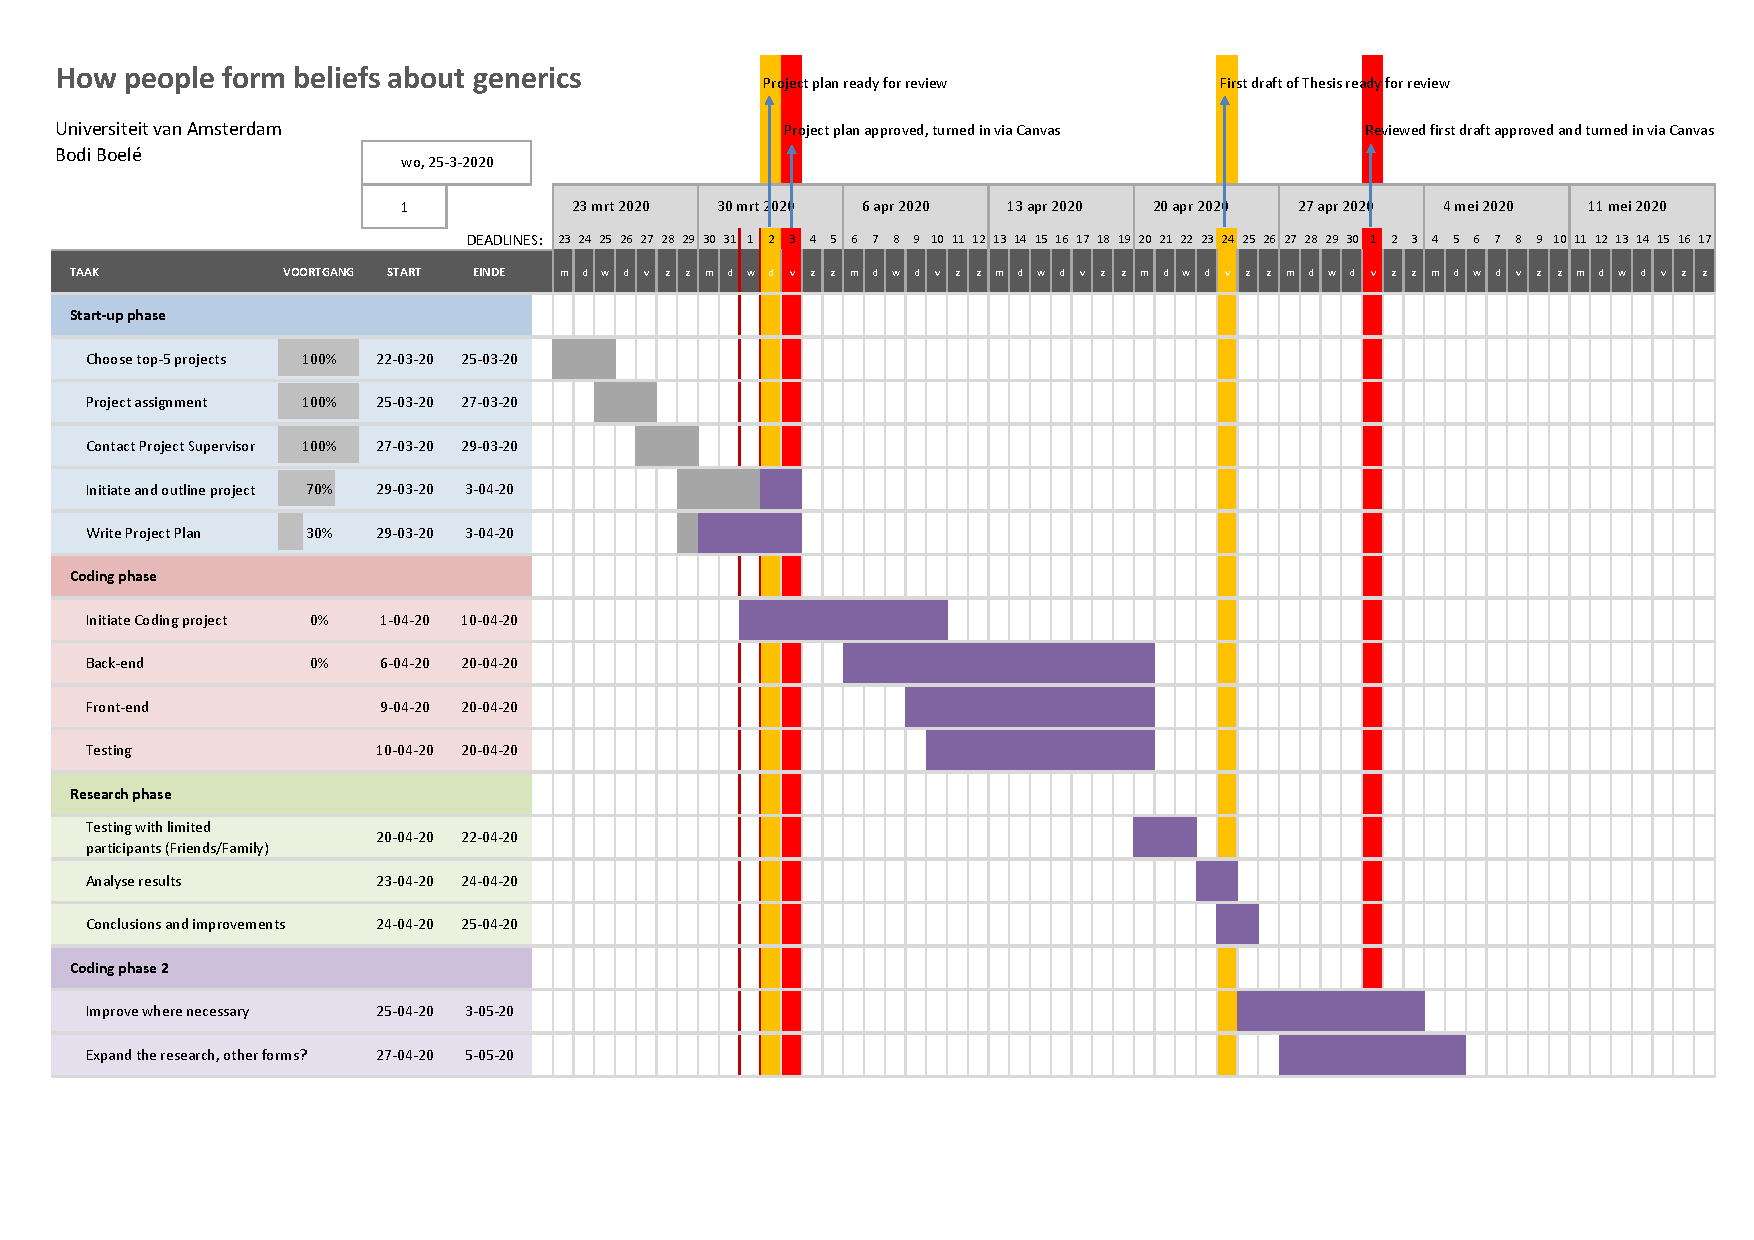
\includepdf[angle=-90, pages=-]{Gant_planning_Afstudeerproject}
%-------------------------------------------------------------------------------
%	EINDE
%-------------------------------------------------------------------------------
\end{document}
